% Options for packages loaded elsewhere
\PassOptionsToPackage{unicode}{hyperref}
\PassOptionsToPackage{hyphens}{url}
\PassOptionsToPackage{dvipsnames,svgnames,x11names}{xcolor}
%
\documentclass[
  english,
  a4paper,
]{article}
\usepackage{amsmath,amssymb}
\usepackage{lmodern}
\usepackage{iftex}
\ifPDFTeX
  \usepackage[T1]{fontenc}
  \usepackage[utf8]{inputenc}
  \usepackage{textcomp} % provide euro and other symbols
\else % if luatex or xetex
  \usepackage{unicode-math}
  \defaultfontfeatures{Scale=MatchLowercase}
  \defaultfontfeatures[\rmfamily]{Ligatures=TeX,Scale=1}
\fi
% Use upquote if available, for straight quotes in verbatim environments
\IfFileExists{upquote.sty}{\usepackage{upquote}}{}
\IfFileExists{microtype.sty}{% use microtype if available
  \usepackage[]{microtype}
  \UseMicrotypeSet[protrusion]{basicmath} % disable protrusion for tt fonts
}{}
\makeatletter
\@ifundefined{KOMAClassName}{% if non-KOMA class
  \IfFileExists{parskip.sty}{%
    \usepackage{parskip}
  }{% else
    \setlength{\parindent}{0pt}
    \setlength{\parskip}{6pt plus 2pt minus 1pt}}
}{% if KOMA class
  \KOMAoptions{parskip=half}}
\makeatother
\usepackage{xcolor}
\IfFileExists{xurl.sty}{\usepackage{xurl}}{} % add URL line breaks if available
\IfFileExists{bookmark.sty}{\usepackage{bookmark}}{\usepackage{hyperref}}
\hypersetup{
  pdftitle={Interaction structure constrains the emergence of conventions in group communication},
  pdflang={en},
  colorlinks=true,
  linkcolor={blue},
  filecolor={Maroon},
  citecolor={blue},
  urlcolor={blue},
  pdfcreator={LaTeX via pandoc}}
\urlstyle{same} % disable monospaced font for URLs
\usepackage[margin=25mm]{geometry}
\usepackage{longtable,booktabs,array}
\usepackage{calc} % for calculating minipage widths
% Correct order of tables after \paragraph or \subparagraph
\usepackage{etoolbox}
\makeatletter
\patchcmd\longtable{\par}{\if@noskipsec\mbox{}\fi\par}{}{}
\makeatother
% Allow footnotes in longtable head/foot
\usepackage{footnote} % For some unknown reason, footnotehyper clashes with French
\makesavenoteenv{longtable}
\usepackage{graphicx}
\makeatletter
\def\maxwidth{\ifdim\Gin@nat@width>\linewidth\linewidth\else\Gin@nat@width\fi}
\def\maxheight{\ifdim\Gin@nat@height>\textheight\textheight\else\Gin@nat@height\fi}
\makeatother
% Scale images if necessary, so that they will not overflow the page
% margins by default, and it is still possible to overwrite the defaults
% using explicit options in \includegraphics[width, height, ...]{}
\setkeys{Gin}{width=\maxwidth,height=\maxheight,keepaspectratio}
% Set default figure placement to htbp
\makeatletter
\def\fps@figure{htbp}
\makeatother
\setlength{\emergencystretch}{3em} % prevent overfull lines
\providecommand{\tightlist}{%
  \setlength{\itemsep}{0pt}\setlength{\parskip}{0pt}}
\setcounter{secnumdepth}{-\maxdimen} % remove section numbering
\newlength{\cslhangindent}
\setlength{\cslhangindent}{1.5em}
\newlength{\csllabelwidth}
\setlength{\csllabelwidth}{3em}
\newlength{\cslentryspacingunit} % times entry-spacing
\setlength{\cslentryspacingunit}{\parskip}
\newenvironment{CSLReferences}[2] % #1 hanging-ident, #2 entry spacing
 {% dont indent paragraphs
  \setlength{\parindent}{0pt}
  % turn on hanging indent if param 1 is 1
  \ifodd #1
  \let\oldpar\par
  \def\par{\hangindent=\cslhangindent\oldpar}
  \fi
  % set entry spacing
  \setlength{\parskip}{#2\cslentryspacingunit}
 }%
 {}
\usepackage{calc}
\newcommand{\CSLBlock}[1]{#1\hfill\break}
\newcommand{\CSLLeftMargin}[1]{\parbox[t]{\csllabelwidth}{#1}}
\newcommand{\CSLRightInline}[1]{\parbox[t]{\linewidth - \csllabelwidth}{#1}\break}
\newcommand{\CSLIndent}[1]{\hspace{\cslhangindent}#1}

%%%%%%%% START HEADER PARTIAL %%%%%%%%%%%%

% Formatting of tables & knitr::kable and kableExtra functionality
\usepackage{float}
\usepackage{colortbl}
\usepackage{pdflscape}
\usepackage{tabu}
\usepackage{threeparttable}

% Line numbering

% endfloat stuff

% fancyhdr pagestyle

% Environment for keywords
\makeatletter
\newcommand\keywordsname{Keywords}
\newenvironment*{keywords}[1][\keywordsname]{\if@twocolumn \else \small \quotation \fi \begin{center} \textbf{\textit{#1} \\}}{\end{center}\if@twocolumn \else \small \endquotation \fi}
\newenvironment*{keywordsinline}[1][\keywordsname]{\if@twocolumn \else \small \quotation \fi \begin{center} \textbf{\textit{#1}: }}{\end{center}\if@twocolumn \else \small \endquotation \fi}
\makeatother

% Environment for abstract that takes new abstract name
\newenvironment{renameableabstract}[1][\abstractname]{\let\oldabstractname\abstractname \renewcommand{\abstractname}{#1} \begin{abstract}}{\end{abstract} \renewcommand{\abstractname}{\oldabstractname}}

%%%%%%%% END HEADER PARTIAL %%%%%%%%%%%%

\usepackage{tikz}
\usetikzlibrary{angles,positioning,arrows.meta, quotes, shapes, shapes.geometric}
\usepackage{graphicx}
\usepackage{booktabs}
\usepackage{longtable}
\usepackage{array}
\usepackage{multirow}
\usepackage{wrapfig}
\usepackage{float}
\usepackage{colortbl}
\usepackage{pdflscape}
\usepackage{tabu}
\usepackage{threeparttable}
\usepackage{threeparttablex}
\usepackage[normalem]{ulem}
\usepackage{makecell}
\usepackage{xcolor}
\ifXeTeX
  % Load polyglossia as late as possible: uses bidi with RTL langages (e.g. Hebrew, Arabic)
  \usepackage{polyglossia}
  \setmainlanguage[]{}
\else
  \usepackage[english,main=english]{babel}
% get rid of language-specific shorthands (see #6817):
\let\LanguageShortHands\languageshorthands
\def\languageshorthands#1{}
\fi
\ifLuaTeX
  \usepackage{selnolig}  % disable illegal ligatures
\fi

\title{Interaction structure constrains the emergence of conventions in group communication}

%%%%%%% START AUTHOR PARTIAL %%%%%%%%%%%%%%%

%%%%% Authors, affiliations and author notes stuff %%%%%

% Macros for creating and referencing stored reference
\makeatletter
\def\MyNewLabel#1#2#3{\expandafter\gdef\csname #1@#2\endcsname{#3}}

\def\MyRef#1#2{\@ifundefined{#1@#2}{???}{\csname #1@#2\endcsname}}

\newcommand*\ifcounter[1]{%
  \ifcsname c@#1\endcsname
    \expandafter\@firstoftwo
  \else
    \expandafter\@secondoftwo
  \fi
}
\makeatother

% Create labels for Addresses if the are given by code
\MyNewLabel{ADDRTXT}{Stanford}{Stanford University}
\MyNewLabel{ADDRTXT}{Princeton}{Princeton University}

% Create labels for Footnotes if they are given by code
\MyNewLabel{ANOTETXT}{corresp}{Corresponding author. Email: \href{mailto:vboyce@stanford.edu}{\nolinkurl{vboyce@stanford.edu}}}

%%% Special footnotes for addresses and author footnotes
\usepackage{bigfoot}
\DeclareNewFootnote{Addr}[arabic] % Only used for NOT authblk
\DeclareNewFootnote{ANote}[fnsymbol]

%%% Address and author notes as a function of format %%%
 % Use authblk for affiliations %%%%%%%%%%%
\usepackage{authblk}

% Always separate by commas
\renewcommand\Authsep{, }
\renewcommand\Authand{, }
\renewcommand\Authands{, }

% Counter for addresses and footnotes
\newcounter{addrcnt}

% thanks definition that doesnt produce superscript marks
\makeatletter
\newcommand*\createaddrlblbycode[1]{%
  \ifcounter{ADDRLBL@#1}
    {}
    {\refstepcounter{addrcnt}\newcounter{ADDRLBL@#1}\setcounter{ADDRLBL@#1}{\value{addrcnt}}}%
}

\newcommand*\addrlblbycode[1]{\arabic{ADDRLBL@#1}}

\newcommand*\addrbycode[1]{%
  \ifcounter{ADDR@#1}
    {}
    {\newcounter{ADDR@#1}%
     \affil[\addrlblbycode{#1}]{\MyRef{ADDRTXT}{#1}}}%
}

\newcommand*\createanotelblbycode[1]{%
  \ifcounter{ANOTELBL@#1}
    {}
    {\refstepcounter{footnoteANote}\newcounter{ANOTELBL@#1}\setcounter{ANOTELBL@#1}{\value{footnoteANote}}}%
}

\newcommand*\anotelblbycode[1]{\fnsymbol{ANOTELBL@#1}}

\newcommand*\anotebycode[1]{%
  \ifcounter{ANOTE@#1}
    {}
    {\newcounter{ANOTE@#1}%
     \footnotetextANote[\value{ANOTELBL@#1}]{\MyRef{ANOTETXT}{#1}}}%
}
\makeatother


\createaddrlblbycode{Stanford}


\createanotelblbycode{corresp}

\author[%
\addrlblbycode{Stanford}%
,%
$\anotelblbycode{corresp}$%
]{Veronica Boyce}

\addrbycode{Stanford}


\createaddrlblbycode{Princeton}



\author[%
\addrlblbycode{Princeton}%
]{Robert Hawkins}

\addrbycode{Princeton}


\createaddrlblbycode{Stanford}



\author[%
\addrlblbycode{Stanford}%
]{Noah D. Goodman}

\addrbycode{Stanford}


\createaddrlblbycode{Stanford}



\author[%
\addrlblbycode{Stanford}%
]{Michael C. Frank}

\addrbycode{Stanford}


%endif(authblk)

%%%%%%%%% END AUTHOR PARTIAL %%%%%%%%

\date{}

\begin{document}
\maketitle

%%%%%%%%%% START AFTER TITLE PARTIAL %%%%%%%%%%%%%
\anotebycode{corresp}


%%%%%%%%%% END AFTER TITLE PARTIAL %%%%%%%%%%%%%


\begin{otherlanguage}{english}

\begin{abstract}
Multi-party communication is ubiquitous, but it presents {[}TODO need more specificity setting up the puzzle: can we say `presents \emph{three key challenges} beyond those faced in dyadic communication' and give them names?{]} some challenges not found in dyadic communication. One test case for communication is iterated reference games, where the phenomenon of reduction over repeated reference is well-attested in dyadic contexts and could explain how pairs of people build shared meanings. We extend the repeated reference game paradigm to groups of 2 to 6 people under varied interaction structure constraints across 313 games (1319 participants). Across conditions, groups shorter their utterances and form shared descriptions. Smaller groups and groups with thicker communication channels converge to shared conventions more rapidly than larger groups with thin communication channels. {[}TODO need another sentence translating this back to the unique challenges of multi-party communication and exposing the relevance of the results for theory/application (e.g.~`Taken together, these results provide new insight into the conditions under which group communication can thrive, with implications for eduction, management, and \ldots{}'){]}

\end{abstract}

\end{otherlanguage}

TODO fix ordering of things on diagrams!

TODO Figure 1 still under discussion!

{[}TODO before jumping in the challenges, I'd start with some examples establishing how ubiquitious it really is. e.g.~``While most psychological studies of communication focus on one-on-one conversations, or dyads, much of our daily lives center around communicating in larger groups. In school, children sit in classrooms with peers and teachers; at home, we have dinner with multiple friends and family; and in the office, we attend meetings with colleagues and managers.' {]}
Communicating in groups can be challenging. Listeners may have different levels of background knowledge that the rest of the groups may be unaware of. Some interlocuters may interrupt with questions, and others might pipe in to explain their views, collectively leading to everyone talking at once. Multiple conversations threads may split off that need to merge back together for the group to reach agreement. Different people may understand the same speaker as meaning different things, resulting in disagreements and misunderstandings. Disagreements may even escalate to the point where meta-discussion is needed to define terms or structure the conversation differently. {[}TODO I'd try to distill each of these down to a noun or short phrase to expose them better as theoretical desiderata (e.g.~`heterogeneity, asynchrony, and clustering' or something. those aren't perfectly descriptive, but that's the idea.){]}

{[}TODO I might rephrase this as `In spite of these considerable challenges, however, speakers are often able to navigate multi-party settings with ease.' (it currently rehashes the argument of the previous paragraph.){]}Conversations with half-a-dozen people can devolve into chaos and result in inefficient communication; yet, other times, we communicate successfully and efficiently with multiple people at once. What aspects of communication channels and interaction structure determine how efficiently a group can communicate?

One key requirement for efficient communication in groups of any size {[}TODO I would incorporate all of the multi-party references from the cogsci paper (and later slack threads) into the earlier paragraphs before jumping to motivating the dyadic paradigm. partly this is just to give credit where credit is due, but also flags that we're entering theoretically and empirically rich ground. {]} is a shared vocabulary, or shared mappings between linguistic units and objects or concepts (\protect\hyperlink{ref-traum2004}{Traum 2004}, \protect\hyperlink{ref-ginzburg2005}{Ginzburg \& Fernandez 2005}, \protect\hyperlink{ref-branigan2006}{Branigan 2006}). {[}TODO maybe need to introduce reference as a particular functional goal of communication before introducing the need for shared vocabulary? it isn't clear that it's going to be the topic of this paragraph, and still needs to be defined.{]} Because reference is a requirement of communication that can be isolated and tested in experimentally manipulated contexts, it has been a case study for efficient communication more broadly. In many cases, ther are widely shared convention mappings between objects and descriptions that people can rely on, but in other cases, interlocuters must invent ad-hoc reference expressions to communicate about objects without canonical names.

The formation of these new reference expressions is well-studied in dyadic contexts. Clark \& Wilkes-Gibbs (\protect\hyperlink{ref-clarkReferringCollaborativeProcess1986}{1986}) established an experimental method for studying the emergence of new referring expressions that has now become standard (building on \protect\hyperlink{ref-kraussChangesReferencePhrases1964}{Krauss \& Weinheimer 1964}, \protect\hyperlink{ref-kraussConcurrentFeedbackConfirmation1966}{1966}). Two participants see the same set of figures; the speaker describes each figure in turn so the listener can select the target from the set of figures. The speaker and listener repeat this process many times with the same images.

Early descriptions are long and make reference to multiple features in the figure, but over the course of the game, shorthand conventional names for each figure emerge; this shortening of utterances is called `reduction'. Not only are later utterances shorter than earlier utterances, but later utterances are a tacitly agreed upon name, understandable within the dyad, but different from the conventions chosen by other dyads.

Recently, online participant recruitment and web-based experiments have made it possible to study this convergence in larger populations (\protect\hyperlink{ref-haber2019}{Haber et al. 2019}, \protect\hyperlink{ref-hawkinsCharacterizingDynamicsLearning2020}{Hawkins et al. 2020}). In line with results from face-to-face, oral paradigms, speakers reduced their utterances, producing fewer words per image in later blocks than in earlier blocks. (Throughout this paper, we use ``speaker'' and ``listener'' to refer to the roles describing and selecting targets, regardless of communication modality.)

What aspects of conversational infrastructure are needed to support this reduction pattern? In the current work, we address how components of interaction structure, including group size and communication channels, shape how successfully groups form partner-specific conventionalized names for target objects over the course of an iterated reference game. We recruited 1319 participants who were organized into 313 groups distributed across 3 online experiments and 11 conditions. Collectively, players produced 326000 words during their games. We analysed the games along 4 metrics: the two traditional metrics of 1) listener accuracy and 2) number of words produced per trial, as well as two computational measures of semantic similarity that addressed 3) how utterances converge towards a conventions with a game and 4) how utterances diverge from descriptions in other games as they become more partner-specific.

\begin{figure*}[t!]

{\centering 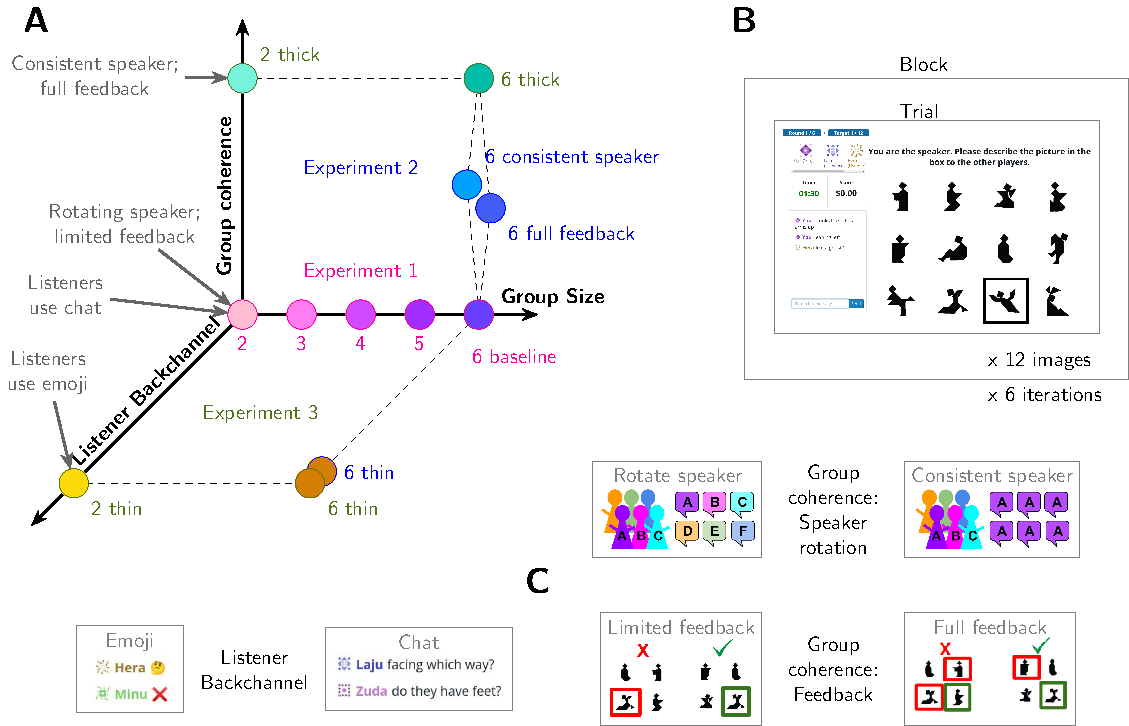
\includegraphics[width=1\linewidth]{expt-diagram} 

}

\caption{A: Diagram of the experimental space explored in these experiments. Experiments varied along 3 dimensions: Group size, group coherence, and listener backchannel. Each condition is shown as a dot. Experiment 1 (pink labels) varied group size from 2-6 players while holding group coherence and backchannel constant. Experiment 2 (blue labels) keep group size constant at 6 and varied the other dimensions. Relative to experiment1, 6 consistent speaker and 6 full feedback each added one component of group coherence, and 6 thin reduced the backchannel. Experiment 3 (green labels) tested 4 corners of the space, crossing group size (2 or 6 players) with thin games (low coherence, low backchannel) or thick games (high coherence, high backchannel). \  B: Each trial a speaker described a target image to the listeners, and this process repeated for all 12 images to comprise a block, and the block repeated for a total of 6 iterations. \ C: Differences between conditions. See text for explanation.}\label{fig:diagram}
\end{figure*}

\hypertarget{results}{%
\section{Results}\label{results}}

{[}TODO need to start with a bit higher-level motivation before jumping into the details (and silly, but don't downplay the originality of the design; it's not just a straightforward extension of earlier designs! motivate it first from first principles and then acknowledge the relationship to earlier designs after.) something like ``We decomposed conversational infrastructure into three elements: {[}\ldots{]}. We then constructed a large-scale chat-room environment where we could systematically manipulate these factors{[}\ldots{]},{]}
We extended on the dyadic paradigm of Hawkins et al. (\protect\hyperlink{ref-hawkinsCharacterizingDynamicsLearning2020}{2020}) by parameterizing the experiments along a few dimensions while keeping other aspects of the experiment constant. As shown in Figure \ref{fig:diagram}B, all of the games used the same 12 target images used in Clark \& Wilkes-Gibbs (\protect\hyperlink{ref-clarkReferringCollaborativeProcess1986}{1986}) and Hawkins et al. (\protect\hyperlink{ref-hawkinsCharacterizingDynamicsLearning2020}{2020}). The speaker knew which image was the target, and their goal was to describe it to the listeners over a chat interface so each listener could select the target. After all listeners had selected, players received feedback on the selections. The process repeated with the same speaker describing each of the 12 images to form one block. The games consisted of 6 blocks, for a total of 72 trials, where each image was described 6 times over the course of the game.

The space of possible iterated reference game experiments is large, but we identified a few dimensions we thought parameterized the experimental space in relevant ways and sampled along these dimensions (\protect\hyperlink{ref-almaatouq2022}{Almaatouq et al. 2022}). The dimensions of variation were game size, speaker rotation, level of feedback, and the form of the listener backchannel. Across the three experiments, we sampled 11 different points in the experimental space, illustrated in Figure \ref{fig:diagram}A.

In experiment 1, we varied the size of the games continuously from \emph{2 to 6 players} while keeping other factors constant to explore what how performance varied across group size. For these conditions, the \emph{speaker role rotated} after each block, so that all players had at least one turn as speaker. We gave \emph{limited feedback} to listeners, showing each listener only whether their individual selection was correct or not, but not revealing other's selections or the right answer. Listeners had access to a \emph{chat box} as their backchannel, so they could freely type questions and offer their own descriptions to the group.

In experiment 2, we explored varying different factors within 6 player games. We tried two different variations that we thought might improve group coherence and lead to better performance: having a \emph{consistent speaker} rather than a rotating speaker, and separately, showing all the listeners \emph{full feedback} on what each person in the group had selected and what the right answer had been. Additionally, we tested the role of listener contributions in establishing mutual understanding with a condition where listeners' backchannel was limited to four \emph{emojis}. Listeners could send 4 discrete messages (green check, thinking face, red x, and laughing-crying face) to the chat. This limited backchannel allowed listeners to convey valence and level of comprehension, but not to contribute any referential content.

In experiment 3, we crossed the extremes of group size from experiment 1 (2 or 6 people) with extremes of group interactions from experiment 2. In the \emph{thick} condition, we combined a consistent speaker with full feedback to create \emph{high group coherence} and let listeners use the chat freely. In the \emph{thin} condition, we repeated the emoji backchannel condition from experiment 2, which had \emph{low group coherence} and an emoji backchannel.

TODO possibly include more justification on why we chose these settings (aka, citations)

We analysed these 3 experiments on 4 key measures: listener accuracy, speaker reduction, convergence of descriptions within games, and divergence of descriptions between games. For analyses, we used a Bayesian multi-level regression framework with weakly regularizing priors (\protect\hyperlink{ref-burkner2018}{Bürkner 2018}); listener accuracy used a logistic regression, all other analyses used linear regression {[}See methods for full priors, and supplement for a full list of models and model results{]}. {[}TODO I like putting the low-level details of the brms calls in the methods/supplement. But in each section below, I think there does need to be some prose description of the regression (e.g.~``We constructed a logistic regression model to predict accuracy in each experiment as a function of the manipulated variable: number of players in the group (Exp.1), thickness of feedback channel (Exp. 2), and the combination of the two (Exp. 3).''{]}

\hypertarget{group-performance}{%
\subsection{Group Performance}\label{group-performance}}

The canonical findings from dyadic reference games are that, over repetitions, listener accuracy is high and increasing while the amount of referential language decreases dramatically. Listener accuracy measures how successful speakers are at communicating the target referent to the listeners. The combination of accuracy and reduction of speaker descriptions indicates that speaker and listeners have formed a shared conceptualization of the target that can be distilled into a shorter form, while still retaining the same level of informativity to listeners.

\begin{figure*}[t!]

{\centering \includegraphics[width=1\linewidth]{figs/behavioral-1} 

}

\caption{Behavioral results across all three experiments. A. Listener accuracy at selecting the target image. Dots are per condition, per block estimates with 95\% bootstrapped CIs. Smooths are binomial fit lines. B. Number of words said by the speaker each trial. Faint dots represent individual trials from individual games. Smooths are quadratic fit lines. Y-axis is truncated, and a few outliers points are not visible. }\label{fig:behavioral}
\end{figure*}

{[}TODO fix footnote{]}

{[}TODO add some numbers for expt 2{]}

\hypertarget{listener-backchanneling-increases-with-group-size}{%
\subsubsection{Listener backchanneling increases with group size}\label{listener-backchanneling-increases-with-group-size}}

In our experiments, listener accuracy rose over repetitions in all conditions and approached ceiling in most conditions; however, 6 player thin games were the least accurate (Figure \ref{fig:behavioral}A). In experiment 1, variation in group size did not have a strong effect on initial accuracy (\(\beta=-0.07,\:95\%\:\mathrm{CrI}=[-0.2, 0.05]\)) or improvement rate (\(\beta=-0.02,\:95\%\:\mathrm{CrI}=[-0.05, 0.01]\)){[}\^{}Throughout, we report the estimate and 95\% credible interval for model coefficients, as well as the model term if it is not obvious from the text.{]}. In experiment 2, accuracy was much higher for consistent speaker and full feedback games than for 6 thin. In experiment 3, the 6 player games had lower initial accuracy (\(\beta=-0.64,\:95\%\:\mathrm{CrI}=[-1.05, -0.25]\)) and were slower to improve (\(\beta=-0.34,\:95\%\:\mathrm{CrI}=[-0.43, -0.25]\)) than the 2 player games. Thin games were not reliably worse than thick games on initial accuracy (\(\beta=-0.36,\:95\%\:\mathrm{CrI}=[-0.78, 0.05]\)) or improvement rate (\(\beta=-0.07,\:95\%\:\mathrm{CrI}=[-0.18, 0.04]\)). The high and increasing levels of accuracy indicate that across all of these conditions, participants are able to succeed in communicating about the images.

\hypertarget{speaker-utterances}{%
\subsubsection{Speaker utterances}\label{speaker-utterances}}

{[}TODO I would make a new subsubsection for this result to make it easier to follow. In this narrative format, you can use subsections liberally (e.g.~it's ok for each paragraph to have its own subsection title, which makes it really easy to read off the structure).{]}
Speakers in larger games were more verbose than speakers in smaller games, and in some cases, these speakers showed sharper reduction from initial wordiness to eventual concision (Figure \ref{fig:behavioral}B). In experiment 1, the overall effect of being one block later was \(\beta=-3.37,\:95\%\:\mathrm{CrI}=[-4.54, -2.24]\) words per trial. Speakers in larger groups said more; the effect of each additional player was \(\beta=1.66,\:95\%\:\mathrm{CrI}=[0.66, 2.61]\) more words per trial, with no clear interaction between block and group size (\(\beta=-0.1,\:95\%\:\mathrm{CrI}=[-0.36, 0.17]\)). In experiment 2, 6 thin had a shallower reduction curve than the other conditions. The result of being one block later was \(\beta=-5.39,\:95\%\:\mathrm{CrI}=[-6.46, -4.31]\) words per trial for 6 consistent speaker; \(\beta=-4.68,\:95\%\:\mathrm{CrI}=[-5.88, -3.52]\) words for 6 full feedback, and \(\beta=-2.15,\:95\%\:\mathrm{CrI}=[-3.44, -1.12]\) words for 6 thin. In experiment 3, the six player games were initially more verbose (\(\beta=7.41,\:95\%\:\mathrm{CrI}=[3.57, 11.18]\)) but reduced faster (\(\beta=-1.21,\:95\%\:\mathrm{CrI}=[-2.06, -0.3]\)) than the two-player games. Thin games were similar to thick games in initial verbosity (\(\beta=0.63,\:95\%\:\mathrm{CrI}=[-3.18, 4.73]\)) and reduction rate (\(\beta=0.32,\:95\%\:\mathrm{CrI}=[-0.65, 1.24]\)).

\hypertarget{listener-utterances}{%
\subsubsection{Listener utterances}\label{listener-utterances}}

Listeners talk much less than speakers, and listener contributions are concentrated in early trials. The more listeners, the more likely it was that some listener talked, and the more listeners said when they talked (CROSSREF SUPPLEMENT IMAGE). In experiment 1, the number of trials where any listener said anything related to the image was higher in larger groups (\(\beta=0.78,\:95\%\:\mathrm{CrI}=[0.58, 0.98]\)) and declined across blocks (\(\beta=-0.8,\:95\%\:\mathrm{CrI}=[-0.97, -0.63]\)). When referential language was produced, larger groups produced more language (\(\beta=2.12,\:95\%\:\mathrm{CrI}=[1.03, 3.12]\)), but the difference in group size closed in later blocks (\(\beta=-0.41,\:95\%\:\mathrm{CrI}=[-0.72, -0.09]\)). This pattern is consistent with early listener involvement in establishing a common conceptualization by asking questions and offering alternative descriptions. Once a shared idea is in place, listener descriptions are rarer and more perfunctory. Emoji use is not directly comparable to referential language, but similar trends occurred in the thin games. Emoji use was more common in the 6 player games than the two player games and decreased over the course of the game (SUPP FIGURE).

{[}TODO: as a higher-level comment: I'd try to catch everywhere we're framing results like this, a backward-looking framing of `traditional metrics' or `classic effects' and instead take ownership of what we found on its own terms. What makes these measures interesting isn't that they were used in earlier studies, what makes them interesting is that they measure the \emph{communicative performance} of the group, and we should emphasize the latter over the former.{]}

According to the traditional metrics of iterated reference games, larger games are similar to smaller games, except with more talking, especially early in the games. Larger groups seem to generally take the time to elaborate descriptions in order for most listeners to understand, especially when listeners can ask specific clarifying questions. This leads to more talking in early rounds for larger games, sometimes followed by sharp reduction once a shared conceptualization is agreed upon.

\hypertarget{linguistic-content}{%
\subsection{Linguistic Content}\label{linguistic-content}}

\begin{figure*}[t!]

{\centering 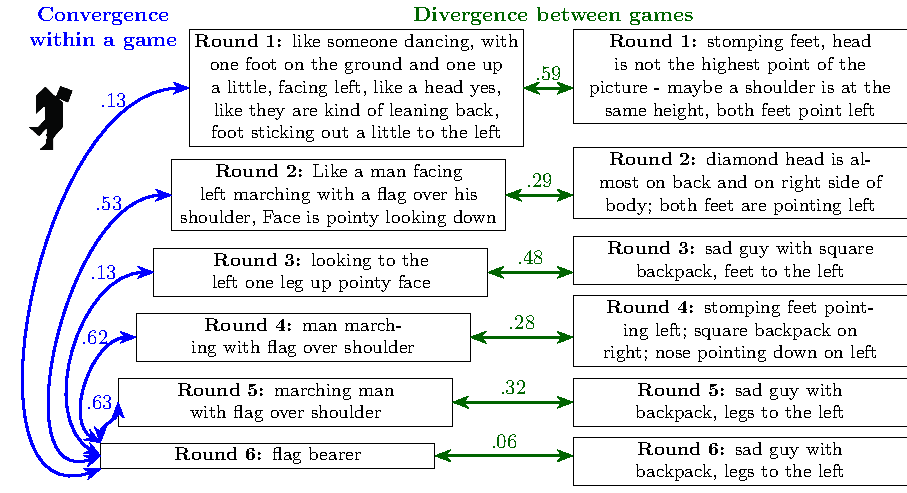
\includegraphics[width=1\linewidth]{sbert} 

}

\caption{Example utterances describing the shown tangram figure produced by two 3-player games in Experiment 1. To measure convergence within a game (blue), we measured the cosine similarity between SBERT embeddings of descriptions and the embedding of the round 6 utterance (taken to be the convention). Higher cosine similarity indicates more similar meaning. To measure divergence between games (green), we measured the similarity between utterances from the same round across games.}\label{fig:sbert-diagram}
\end{figure*}

{[}TODO: i'd try to start this paragraph off with a set of hypotheses similar to the way we tried to originally motivate these analyses in terms of `arbitrariness' and `stability', but in this case trying to deepen particular patterns we observed across different group sizes and feedback channels (e.g.~`there are a number of reasons larger group may reduce to more efficient referring expressions when thicker feedback is available. one possibility is that these speakers simply get bored of the task faster and lose track of their own idiosyncratic labels, saying something different every block. another possibility is that there is a universal 'best' label for every tangram, and those speakers are better able to discover it. A final possibility is that each group coordinates on their own idiosyncratic conventions but those speakers are better able to pool the group's feedback. To distinguish between these possibilities, we turn to the linguistic content of the utterances. In particular, we examine the \emph{semantic similarity} of descriptions within and across games.'{]}
The reduction in words is a signal of the formation of a partner-specific conceptualization of the target image, but the formation of partner-specific shorthands can be measured more directly by looking at shifts in the semantic similarity of descriptions. As a group converges to a nickname for a target, descriptions within a game, to the same target, become more similar to each other and to the eventual convention. At the same time, as different groups latch onto different features as the key concept, descriptions of the same image from different groups decrease in similarity over time.

These two key trends occurred across conditions, but were much weaker in the 6-player thin games than in other conditions. We quantified description similarity by concatenating speaker messages together within a trial and embedding this description into a high-dimensional vector space using SBERT (\protect\hyperlink{ref-reimers2019}{Reimers \& Gurevych 2019}). Then, we compared the similarity between pairs of utterances by taking the cosine similarity between their embeddings. Figure \ref{fig:sbert-diagram} shows an example of concatenated utterances and their cosine similarities.

\begin{figure*}[t!]

{\centering \includegraphics[width=1\linewidth]{figs/sbert-1} 

}

\caption{Language similarity results measured with pairwise cosine similarity between embeddings of two utterances. A. Convergence of utterances within games as measured by similarity between an utterance from block 1-5 to the block 6 utterance in the same game for the same image. Dots are per-game averages, smooths are quadratic. B. Divergence of utterances across games as measured by the similarity between an utterances and utterances produced for the same image by different groups in the same block. Dots are per-image averages, smooths are quadratic.}\label{fig:sbert}
\end{figure*}

Speaker descriptions converged toward the final description across conditions; convergence was fastest in smaller and higher coherence groups, and was least strong in the 6-player thin condition (Figure \ref{fig:sbert}A). In experiment 1, the similarity of the first utterance to the last utterance was invariant across group size (\(\beta=-0.008,\:95\%\:\mathrm{CrI}=[-0.021, 0.005]\)), but smaller groups converged faster (\(\beta=-0.008,\:95\%\:\mathrm{CrI}=[-0.011, -0.005]\)). In experiment 2, convergence was especially rapid for the consistent speaker condition (\(\beta=0.086,\:95\%\:\mathrm{CrI}=[0.078, 0.094]\)) where all the utterances come from the same person. In experiment 3, convergence was slower in thin games than thick games (\(\beta=-0.025,\:95\%\:\mathrm{CrI}=[-0.033, -0.017]\)) and especially thin 6 player games (\(\beta=-0.035,\:95\%\:\mathrm{CrI}=[-0.047, -0.025]\)). Convergence towards the last utterance was driven by cumulative increasing similarity between pairs of utterances in adjacent blocks, as shown in Figure SUPP TODO and model results in SUPPLEMENT.

Over repetitions, speaker descriptions diverged from descriptions used in other groups: divergence was fastest in groups with thick communication channels, while the 6-player thin condition games barely diverged at all (Figure \ref{fig:sbert}B). In experiment 1, cross-group similarities started off the same regardless of group size (\(\beta=0.002,\:95\%\:\mathrm{CrI}=[0, 0.004]\)), but larger groups diverged from each other slightly slower than smaller groups (\(\beta=0.001,\:95\%\:\mathrm{CrI}=[0.001, 0.002]\)). In experiment 2, divergence was stronger in the consistent speaker (\(\beta=-0.041,\:95\%\:\mathrm{CrI}=[-0.043, -0.039]\)) and full feedback conditions (\(\beta=-0.038,\:95\%\:\mathrm{CrI}=[-0.04, -0.035]\)) than in the 6 thin condition (\(\beta=-0.004,\:95\%\:\mathrm{CrI}=[-0.006, -0.001]\)). In experiment 3, the 2-player thick condition diverged at a moderate speed (\(\beta=-0.024,\:95\%\:\mathrm{CrI}=[-0.025, -0.023]\)), and the 6-player thick condition had initially higher similarity (\(\beta=0.051,\:95\%\:\mathrm{CrI}=[0.047, 0.055]\) and faster divergence (\(\beta=-0.008,\:95\%\:\mathrm{CrI}=[-0.01, -0.007]\) in comparison. Compared to the two-player thick games, two-player thin games started with slightly higher similarity (\(\beta=0.014,\:95\%\:\mathrm{CrI}=[0.01, 0.018]\)) and diverged slightly more slowly (\(\beta=0.004,\:95\%\:\mathrm{CrI}=[0.002, 0.005]\)). Most noticeably, the 6 player thin games diverged much more slowly than the other conditions (\(\beta=0.017,\:95\%\:\mathrm{CrI}=[0.015, 0.019]\)).

{[}TODO citation!{]} Theoretical approaches treat reduction and partner-specific convention formation as synonymous, but these measures come apart in the 6 player thin condition. The 6-player thin games show much less divergence between games and convergence within games, even compared to the 2 thin and 6 thick conditions, but 6 player thin games showed smaller (and statistically inconconclusive) differences to 6 thick games for accuracy and reduction. This gap between the traditional measures and the semantic measures raises the possibility that it is possible to become more concise (and more accurate) without developing group-specific nicknames, but instead perhaps relying on group priors and reducing the amount of detail (\protect\hyperlink{ref-guilbeault2021}{Guilbeault et al. 2021}). This gap highlights the need to use measures of the type of language (and not just amount of language) when looking for convention-formation phenomena.

\hypertarget{general-discussion}{%
\section{General Discussion}\label{general-discussion}}

Communication often occurs in multi-party settings, but research on referential communication often does not. In dyadic work, iterated reference games have been used to establish a phenomena of reduction over repeated reference, characterized by speaker-listener pairs creating short nicknames that they mutually understand, but which are not shared by other groups. In this work, we asked how this process of reference formation unfolds under varying interaction structures.

Across 3 online experiments and 11 experimental conditions, we varied game features including group size, form of listener backchannel, and degree of group coherence. All conditions showed the hallmarks of reduction: increasing accuracy, reduction in speaker utterances, semantic convergence within games, and differentiation of descriptions between groups. Even with larger groups and more constrained means of communication, reduction still occurs.

However, while results are directionally the same across conditions, the interaction structure of a group substantially affects how rapidly groups develop partner-specific conventions. Smaller groups and games with thicker communication channels converged faster and more robustly than games that were larger or had thinner communication channels. These factors add together to form the overall group experience. The differences between the 6 player thin condition and both the 2 player thin condition and other 6 player conditions point to an interaction: 2-player games can cope with limited feedback mechanisms, but 6-player games suffer without access to more feedback. Group dynamics differ depending on group size, and larger groups may be more sensitive to other factors affecting interaction structure. Multi-player groups thus make for a richer and more sensitive environment to study communication phenomena applicable to both pairs and small groups.

Just within the general framework of iterated reference, there is a high dimensional feature space of possible experiments. We sampled only a few points along a few dimensions in the space that felt salient. In our experiment 3, we grouped some factors together in order to have more games in each condition: a fully factorial design would have been too expensive to power adequately. Future work could sample other points in the experimental space, perhaps exploring the effects of different target images, or groups of people with real-life prior connections.

We cannot make claims about causal mechanisms between how experimental set-ups such as group size resulted in different outcomes: for instance, there are many differences between being in a 2-person group versus a 6-person group that could lead to the different outcomes. In a dyad, speakers can tailor their utterances to the one listener, but in large groups, speakers must balance the competing needs of different listeners (\protect\hyperlink{ref-schober1989}{Schober \& Clark 1989}, \protect\hyperlink{ref-tolins2016}{Tolins \& Fox Tree 2016}). These effects likely vary by both the knowledge state of and communication channels available to the listeners (\protect\hyperlink{ref-horton2002}{Horton \& Gerrig 2002}, \protect\hyperlink{ref-horton2005}{Horton \& Gerrig 2005}, \protect\hyperlink{ref-fox-tree2013}{Fox Tree \& Clark 2013}). Further work digging into the language used and the interactions between participants might unearth plausible mechanisms for how differences in group size and interaction structure influence outcomes, and this in turn could then point towards future experimental conditions.

\hypertarget{methods}{%
\section{Methods}\label{methods}}

For all experiments, we used Empirica (\protect\hyperlink{ref-almaatouqEmpiricaVirtualLab2020}{Almaatouq et al. 2020}) to create real-time multi-player iterated reference games. In each game, one of the players started as the speaker who saw an array of tangrams with one highlighted and communicated which figure to click to the other players (listeners). After the speaker had identified each of the 12 images in turn, the process repeated with the same images, but a total of 6 blocks (72 trials). We recorded what participants said in the chat, as well as who selected what image and how long they took to make their selections.

These experiments were designed sequentially and pre-registered individually.\footnote{Experiment 1: \url{https://osf.io/cn9f4} for the 2-4 player groups, and \url{https://osf.io/rpz67} for the 5-6 player data run later. Experiment 2: consistent speaker at \url{https://osf.io/f9xyd}, full feedback at \url{https://osf.io/j5zbm}, and thin at \url{https://osf.io/k5f4t}. Experiment 3: \url{https://osf.io/untzy}} We followed the analysis plan, although additional analyses were added to early experiments that were only pre-registered in later experiments. Results from some pre-registered models were omitted from the main text, but are shown in the supplement TODO.

\hypertarget{participants}{%
\subsection{Participants}\label{participants}}

Participants were recruited using the Prolific platform, and all participants self-reported as fluent native English speakers on Prolific's demographic prescreen. Participants each took part in only one experiment. Experiment 1 took place between May and July 2021, experiment 2 between March and August 2022, and experiment 3 in October 2022. As games varied in length depending on the number of participants, we paid participants based on group size, with the goal of a \$10 hourly rate. Participants were paid \$7 for 2-player games, \$8.50 for 3-player games, \$10 for 4-player games, and \$11 for 5- and 6-player games. When one player had the speaker role for the entirety of a 6-player game, they gained an addition \$2 bonus. Across all games, each participant could early up to \$2.88 in performance bonuses. A total of 1319 people participated across the 3 experiments, for roughly 20 games in each condition in experiments 1 and 2 and 40 games per condition in experiment 3. A breakdown of number of games and participants in each condition is shown in TODO supplement.

\hypertarget{materials}{%
\subsection{Materials}\label{materials}}

We used the 12 tangram images used by Hawkins et al. (\protect\hyperlink{ref-hawkinsCharacterizingDynamicsLearning2020}{2020}) and Clark \& Wilkes-Gibbs (\protect\hyperlink{ref-clarkReferringCollaborativeProcess1986}{1986}). These images were displayed in a grid with order randomized for each participant (thus descriptions such as ``top left'' were ineffective as the image might be in a different place on the speaker's and listeners' screens). The same images were used every block.

\hypertarget{procedure}{%
\subsection{Procedure}\label{procedure}}

The experimental procedure was very similar across the three experiments. We first describe the procedure used in experiment 1 and then describe the differences in later experiments.

\hypertarget{experiment-1}{%
\subsubsection{Experiment 1}\label{experiment-1}}

From Prolific, participants were directed to our website where they navigated through a self-paced series of instruction pages explaining the game. Participants had to pass a quiz to be able to play the game. They were then directed to a ``waiting room'' screen until their partner(s) were ready.

Each trial, the speaker described the highlighted tangram image so that the listeners could identify and click it. All participants were free to use the chat box to communicate, but listeners could only click once the speaker had sent a message. Once a listener clicked, they could not change their selection. There was no signal to the speaker or other listeners about who had already made a selection.

Once all listeners had selected (or a 3-minute timer ran out), participants were given feedback. Listeners learned whether they individually had chosen correctly or not; listeners who were incorrect were not told the correct answer. The speaker saw which tangram each listener had selected, but listeners did not. Listeners got 4 points for each correct answer; the speaker got points equal to the average of the listeners' points. These points translated into performance bonus at the end of the experiment.

In each block, each of the 12 tangrams was indicated to the speaker once. The same person was the speaker for an entire block, but participants rotated roles between blocks. Thus, over the course of the 6 blocks, participants were speakers 3 times in 2-player games, twice in 3-player games, once or twice in 4 and 5-player games, and once in 6-player games. Rotating the speaker was chosen to keep participants more equally engaged (the speaker role is more work), and to give a more robust test for reduction and convention.

After the game finished, participants were given a survey asking for optional demographic information and feedback on their experience with the game.

\hypertarget{differences-in-experiment-2}{%
\subsubsection{Differences in experiment 2}\label{differences-in-experiment-2}}

Experiment 2 consisted of three different variations on Experiment 1, all conducted in 6 player games. Each of these conditions differed from the experiment 1 baseline in one way. The consistent speaker condition differed only in that one person was designated the speaker for the entire game, rather than having the speaker role rotate. The full feedback condition differed from experiment 1 in that all participants were shown what each person had selected and what the right answer was; listeners still saw text saying whether they individually were right or wrong. This was similar to some dyadic work, such as Hawkins et al. (\protect\hyperlink{ref-hawkinsCharacterizingDynamicsLearning2020}{2020}) where listeners were shown what the right answer was during feedback. For the thin condition, we altered the chatbox interface for listeners. Instead of a textbox, listeners had 4 buttons, each of which sent a different emoji to the chat. Listeners were given suggested meanings for the 4 emojis during instructions. They could send the emojis as often as desired, for instance, initially indicating confusion, and later indicating understanding. In addition, we added notifications that appeared in the chat box saying when a player had made a selection.

\hypertarget{differences-in-experiment-3}{%
\subsubsection{Differences in experiment 3}\label{differences-in-experiment-3}}

The thin channel condition in experiment 3 was the same as the thin condition in experiment 2, above. The thick condition combined the two group coherency enhancing variations from experiment 2: one person was the designated speaker throughout, and the feedback participants received included the right answer and what each player had selected. Across both conditions in experiment 3, notifications were sent to the chat to indicate when a participant had made a selection.

\hypertarget{data-pre-processing-and-exclusions}{%
\subsection{Data pre-processing and exclusions}\label{data-pre-processing-and-exclusions}}

Participants could use the chat box freely, which meant that the chat transcript contained some non-referential language. The first author skimmed the chat transcripts, tagging utterances that did not refer to the current tangram. These were primarily pleasantries (``Hello''), meta-commentary about how well the task was going, and confirmations or denials (``ok'', ``got it'', ``yes'', ``no''). We excluded these utterances from our analyses. Note that chat lines sometimes included non-referential words in addition to words referring to the tangrams (``ok, so it looks like a zombie'', ``yes, the one with legs''); these lines were retained intact.

In experiments 1 and 2, games did not start if there were not enough participants and ended if any participant disconnected. In experiment 3, games started after a waiting period even if they were not full and continued even after a participant disconnected (with speaker role reassigned if necessary), unless the game would drop below 2 players. The distribution of players in these 6* player games is at TODO SUPPLEMENT! The realities of online recruitment and disconnection meant that the number of games varied between conditions. We excluded incomplete blocks from analyses, but included complete blocks from partial games (See SUPPLEMENT TABLE for counts).

When skimming transcripts to tag non-referential utterances, we noticed that one game in the 6-player thick game had a speaker who did not give any sort of coherent descriptions, even with substantial listener prompting. We excluded this game from analyses.

\hypertarget{modelling-strategy}{%
\subsection{Modelling strategy}\label{modelling-strategy}}

In experiment 3, some of the 6 player games did not have 6 players for the entire game. We do not model this, as it is unclear at what point in the game group size is most relevant. We note that this is a conservative choice that will underestimate differences between 2 player and (genuine) 6 player games, by labelling some smaller groups as 6 player.

We ran all models in BRMS (\protect\hyperlink{ref-burkner2018}{Bürkner 2018}) with weakly regularizing priors. We were often unable to fit the full mixed effects structure that we had pre-registered in a reasonable amount of time, so we included what heirarchical effects were reasonable. (All model results and priors and formulae are reported in TODO supplement). Accuracy models were run as logistic models with normal(0,1) priors for both betas and sd. Reduction models were run as linear models with an intercept prior of normal(12,20), a beta prior of normal(0,10), an sd prior of normal(0,5) and a correlation prior of lkj(1). For all of the models of sbert similarity, we used linear models with the priors normal(.5,.2) for intercept, normal(0,.1) for beta, and normal(0,.05) for sd.

\hypertarget{references}{%
\section{References}\label{references}}

\setlength{\parindent}{-0.1in} 
\setlength{\leftskip}{0.125in}

\noindent

\hypertarget{refs}{}
\begin{CSLReferences}{1}{0}
\leavevmode\vadjust pre{\hypertarget{ref-almaatouqEmpiricaVirtualLab2020}{}}%
Almaatouq A, Becker J, Houghton JP, Paton N, Watts DJ, Whiting ME (2020) \href{http://arxiv.org/abs/2006.11398}{Empirica: A virtual lab for high-throughput macro-level experiments}. \emph{ArXiv200611398 Cs}

\leavevmode\vadjust pre{\hypertarget{ref-almaatouq2022}{}}%
Almaatouq A, Griffiths TL, Suchow JW, Whiting ME, Evans J, Watts DJ (2022) Beyond {Playing} 20 {Questions} with {Nature}: {Integrative Experiment Design} in the {Social} and {Behavioral Sciences}. \emph{Behavioral and Brain Sciences}:1--55. doi:\href{https://doi.org/10.1017/S0140525X22002874}{10.1017/S0140525X22002874}

\leavevmode\vadjust pre{\hypertarget{ref-branigan2006}{}}%
Branigan H (2006) Perspectives on multi-party dialogue. \emph{Research on Language and Computation} \textbf{4}:153--177

\leavevmode\vadjust pre{\hypertarget{ref-burkner2018}{}}%
Bürkner P-C (2018) Advanced bayesian multilevel modeling with the r package brms. \emph{The R Journal} \textbf{10}:395--411

\leavevmode\vadjust pre{\hypertarget{ref-clarkReferringCollaborativeProcess1986}{}}%
Clark HH, Wilkes-Gibbs D (1986) \href{http://www.speech.kth.se/~edlund/bielefeld/references/clark-and-wilkes-gibbs-1986.pdf}{Referring as a collaborative process}. \emph{Cognition}

\leavevmode\vadjust pre{\hypertarget{ref-fox-tree2013}{}}%
Fox Tree JE, Clark NB (2013) Communicative {Effectiveness} of {Written Versus Spoken Feedback}. \emph{Discourse Processes} \textbf{50}:339--359. doi:\href{https://doi.org/10.1080/0163853X.2013.797241}{10.1080/0163853X.2013.797241}

\leavevmode\vadjust pre{\hypertarget{ref-ginzburg2005}{}}%
Ginzburg J, Fernandez R (2005) Action at a distance: The difference between dialogue and multilogue. \emph{Proceedings of DIALOR}:9

\leavevmode\vadjust pre{\hypertarget{ref-guilbeault2021}{}}%
Guilbeault D, Baronchelli A, Centola D (2021) Experimental evidence for scale-induced category convergence across populations. \emph{Nat Commun} \textbf{12}:327. doi:\href{https://doi.org/10.1038/s41467-020-20037-y}{10.1038/s41467-020-20037-y}

\leavevmode\vadjust pre{\hypertarget{ref-haber2019}{}}%
Haber J, Baumgärtner T, Takmaz E, Gelderloos L, Bruni E, Fernández R (2019) The {PhotoBook Dataset}: {Building Common Ground} through {Visually-Grounded Dialogue}. In: \emph{Proc. 57th {Annu}. {Meet}. {Assoc}. {Comput}. {Linguist}.} {Association for Computational Linguistics}, {Florence, Italy}, p 1895--1910. Available from: \url{https://www.aclweb.org/anthology/P19-1184} {[}Last accessed 1 February 2022{]}. doi:\href{https://doi.org/10.18653/v1/P19-1184}{10.18653/v1/P19-1184}

\leavevmode\vadjust pre{\hypertarget{ref-hawkinsCharacterizingDynamicsLearning2020}{}}%
Hawkins RD, Frank MC, Goodman ND (2020) \href{http://arxiv.org/abs/1912.07199}{Characterizing the dynamics of learning in repeated reference games}. \emph{ArXiv191207199 Cs}

\leavevmode\vadjust pre{\hypertarget{ref-horton2002}{}}%
Horton WS, Gerrig RJ (2002) {SpeakersÕ} experiences and audience design: Knowing when and knowing how to adjust utterances to addresseesq. \emph{Journal of Memory and Language}:18

\leavevmode\vadjust pre{\hypertarget{ref-horton2005}{}}%
Horton WS, Gerrig RJ (2005) The impact of memory demands on audience design during language production. \emph{Cognition} \textbf{96}:127--142. doi:\href{https://doi.org/10.1016/j.cognition.2004.07.001}{10.1016/j.cognition.2004.07.001}

\leavevmode\vadjust pre{\hypertarget{ref-kraussChangesReferencePhrases1964}{}}%
Krauss RM, Weinheimer S (1964) Changes in reference phrases as a function of frequency of usage in social interaction: A preliminary study. \emph{Psychon Sci} \textbf{1}:113--114. doi:\href{https://doi.org/10.3758/BF03342817}{10.3758/BF03342817}

\leavevmode\vadjust pre{\hypertarget{ref-kraussConcurrentFeedbackConfirmation1966}{}}%
Krauss RM, Weinheimer S (1966) Concurrent feedback, confirmation, and the encoding of referents in verbal communication. \emph{Journal of Personality and Social Psychology} \textbf{4}:343--346. doi:\href{https://doi.org/10.1037/h0023705}{10.1037/h0023705}

\leavevmode\vadjust pre{\hypertarget{ref-reimers2019}{}}%
Reimers N, Gurevych I (2019) Sentence-{BERT}: {Sentence Embeddings} using {Siamese BERT-Networks}. doi:\href{https://doi.org/10.48550/arXiv.1908.10084}{10.48550/arXiv.1908.10084}

\leavevmode\vadjust pre{\hypertarget{ref-schober1989}{}}%
Schober MF, Clark HH (1989) Understanding by addressees and overhearers. \emph{Cognitive Psychology} \textbf{21}:211--232. doi:\href{https://doi.org/10.1016/0010-0285(89)90008-X}{10.1016/0010-0285(89)90008-X}

\leavevmode\vadjust pre{\hypertarget{ref-tolins2016}{}}%
Tolins J, Fox Tree JE (2016) Overhearers {Use Addressee Backchannels} in {Dialog Comprehension}. \emph{Cogn Sci} \textbf{40}:1412--1434. doi:\href{https://doi.org/10.1111/cogs.12278}{10.1111/cogs.12278}

\leavevmode\vadjust pre{\hypertarget{ref-traum2004}{}}%
Traum D (2004) Issues in {Multiparty Dialogues}. In: Dignum F (ed) \emph{Advances in {Agent Communication}}. {Springer Berlin Heidelberg}, {Berlin, Heidelberg}, p 201--211. Available from: \url{http://link.springer.com/10.1007/978-3-540-24608-4_12} {[}Last accessed 1 February 2022{]}. doi:\href{https://doi.org/10.1007/978-3-540-24608-4_12}{10.1007/978-3-540-24608-4\_12}

\end{CSLReferences}


\end{document}
